\documentclass[12pt]{article}
\usepackage[paper=letterpaper,margin=1.5cm]{geometry}
\usepackage{amsmath,amssymb,amsfonts}
\usepackage{newtxtext, newtxmath}
\usepackage{enumitem}
\usepackage{titling}
\usepackage[colorlinks=true]{hyperref}

\usepackage{listings}
\usepackage[font=small,labelfont=bf]{caption} % Required for specifying captions to tables and figures

\usepackage{graphicx} % Required for the inclusion of images
\graphicspath{{./images/}} % Specifies the directory where pictures are stored

\setlength{\droptitle}{-6em}

\begin{document}

\center
Aprendizagem 2024\\
Homework I -- Group 016\\
(ist1106022, ist1106720)\vskip 1cm

\large{\textbf{Part I}: Pen and paper}\normalsize
\begin{enumerate}[leftmargin=\labelsep, label=\textbf{\arabic*.)}]
    \item FILL ME
    \item FILL ME
    \item FILL ME
    \item FILL ME
\end{enumerate}


\large{\textbf{Part II}: Programming}\normalsize
\begin{enumerate}[leftmargin=\labelsep, label=\textbf{\arabic*.)},start=5]
    \item To compare the performance of a Linear Regression Model and two MLP Regressors with 2 hidden layers of 10 neurons each, except one has no activation function while the other has ReLU activation functions, we averaged out the performance of each model over 10 separate runs on different 80-20 train-test splits. The resulting boxplots for each model are:

          \begin{center}
              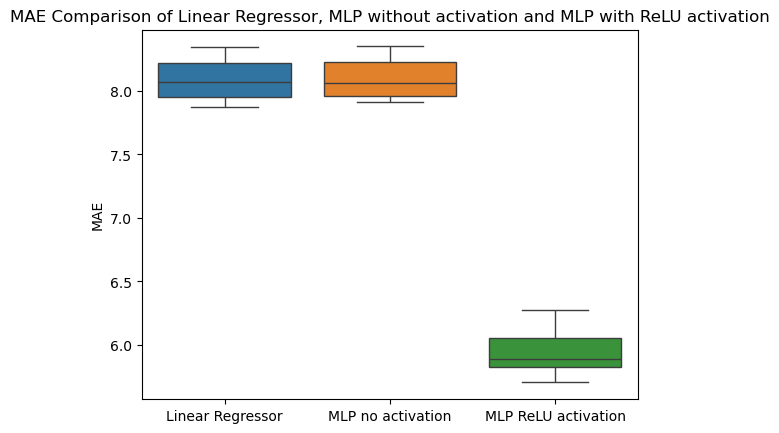
\includegraphics[width=0.8\textwidth]{boxplot_models_MAE.png}
              \captionof{figure}{Boxplot graphs for the Mean Absolute Error of different regression models, accross 80-20 train-test splits.}
          \end{center}

    \item As expected the Linear and MLP without activation regressors have high similar absolute errors, since they can only be used in linearly separable datasets. By adding an activation function, such as ReLU, on the MLP model we are able to learn non-linear patterns within the dataset, which obviously results in a lower absolute error.

          The reason that no activation function, which in reality is the default sign function, leads to bad results is because it creates a linear decision boundary, which is not suitable for non-linear datasets, that can't be separated by simple lines, but rather complex non-linear boundaries.

    \item MLP regressors have varied hyperparameters that can be tuned to improve their performance. To find the best combination of hyperparameters, within the choices presented in the assignment, we used a grid search approach, with a single split, applied on all combinations. The results were as follows:

          \begin{center}
              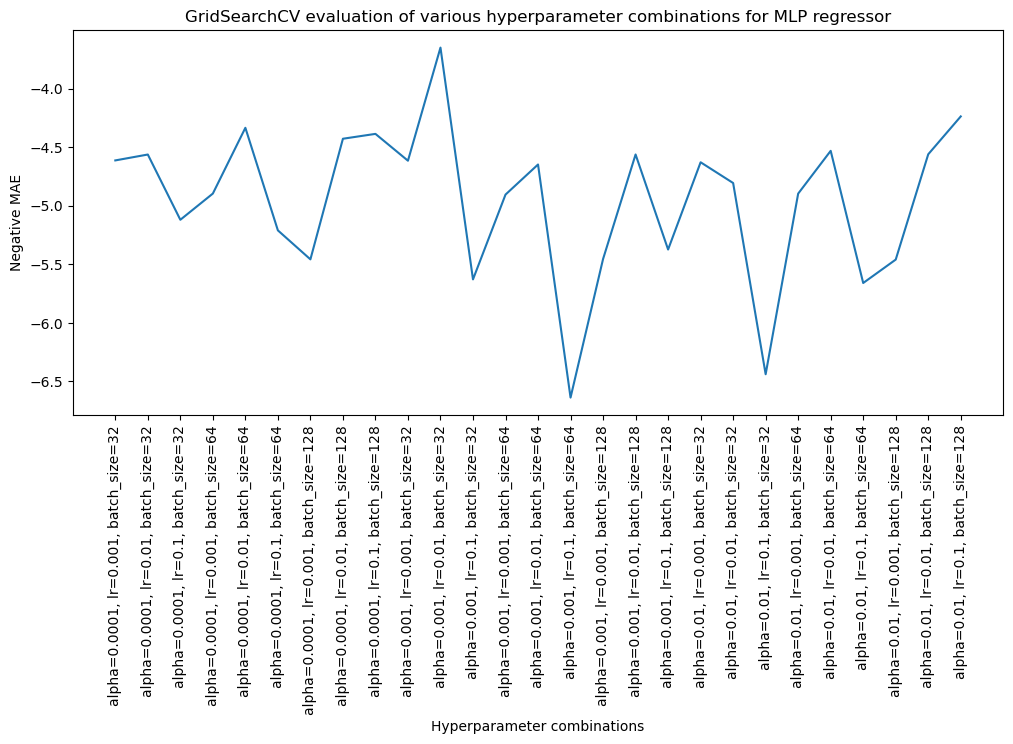
\includegraphics[width=0.8\textwidth]{hyperparameters_performance_plot.png}
              \captionof{figure}{Performance of different hyperparameters combinations on the MLP Regressor}
          \end{center}

          As it can be seen on the plot, the best L2 penalty - Learning Rate - Batch size combination is the one that leads to the lowest Mean Absolute Error, which is the following combination:

            \begin{itemize}
                \item L2 penalty: 0.001
                \item Learning Rate: 0.01
                \item Batch Size: 32
            \end{itemize}
        
            MISSING: DISCUSSION OF TRADE-OFFS BETWEEN COMBINATIONS
\end{enumerate}
\end{document}
